% used class: memoir and in article form for headers etc.
\documentclass[11pt, a4paper, oneside, article]{memoir}

% Inhaltsverzeichnis:
\usepackage{hyperref} %for hyperlinks
\maxtocdepth{subsection} %for depth in contents
\usepackage{amssymb}

%subsection numbering showed:
\setsecnumdepth{subsection}

% Font: Arial
\usepackage{helvet}
\renewcommand{\familydefault}{\sfdefault}

% wenn unbekannte Silbentrennung dann in nächste zeile und große abstände
\sloppy

%Zeilenabstand:
\OnehalfSpacing

%Abstände zum Rand: (gestochen scharf will 2cm)
\setlrmarginsandblock{2.5cm}{2cm}{*}
\setulmarginsandblock{2cm}{*}{1}
\checkandfixthelayout

%Inserting Images:
\usepackage{graphicx}
\graphicspath{ {./images/} {./schematics} {../Setup/Aufnahmen} {../Setup/Arbeitsbereich}}

%For Highlighting Commands
\usepackage{listings}
\lstset{basicstyle=\tiny}

%Bibliography: APA
\usepackage[nosectionbib]{apacite}
\bibliographystyle{apacite}

%Equations
\usepackage{amsmath}

%Including PDFs
\usepackage{pdfpages}

%Für plots
% \usepackage{filecontents} % um eine csv datei zu lesen
\usepackage{pgfplotstable}
\pgfplotsset{compat=1.17}
\usepackage{siunitx}
\usepackage{booktabs} % For \toprule, \midrule and \bottomrule
\usepgfplotslibrary{units} % Allows to enter the units nicely
% geometrische Formen: tikz
% \sisetup{
%   round-mode          = places, % Rounds numbers
%   % round-precision     = 2, % to 2 places/
% }
%Für Anführungszeichen
\usepackage[autostyle=true,german=quotes]{csquotes}

%Abkürzungsverzeichnis
\usepackage[acronym,nonumberlist,nopostdot]{glossaries}
\makenoidxglossaries
% \newacronym{hmd}{HMD}{Head Mounted Display}

\renewcommand{\acronymname}{Abkürzungsverzeichnis}
\glstoctrue

%Tables:
% \renewcommand{\arraystretch}{1.5} %Für mehr Abstand in Tabellen

% \vspace{20pt}
% 
\includegraphics[scale=0.07]{Logo_Uni-Kassel.png}\vspace{50pt}
% \begin{center}
% \large\textbf{Universität Kassel}\\
% Fachbereich 16\\
% \large Mechatronik\\\vspace{50pt}
% \Large\textbf{Literature Research}\\
% \Large\textbf{Representation Learning for Zero-Shot Anomaly Detection}\\
% \vspace{120pt}
% \large
% \begin{tabular}{rl}
% Supervisor: & M. Mgt. Chandana Priya Nivarthi\\
%   & \\
% Author: & Johannes Hölker\\
%  & Matr.-Nr. 35192059\\
%  & johannes.hoelker@uni-kassel.de\\\vspace{40pt}
%  & \\
%  & \\
%  & Cassel, \\
% \end{tabular}
% \end{center}
% \thispagestyle{empty}
%
\title{Representation Learning for Zero-Shot Anomaly Detection}
%
%\titlerunning{Abbreviated paper title}
% If the paper title is too long for the running head, you can set
% an abbreviated paper title here
%
\author{Johannes Hölker\inst{1}\orcidID{0000-1111-2222-3333}} %\and
% Second Author\inst{2,3}\orcidID{1111-2222-3333-4444} \and
% Third Author\inst{3}\orcidID{2222--3333-4444-5555}}
%
\authorrunning{J. Hölker}
% First names are abbreviated in the running head.
% If there are more than two authors, 'et al.' is used.
%
\institute{University of Cassel, Princeton NJ 08544, USA \and
Springer Heidelberg, Tiergartenstr. 17, 69121 Heidelberg, Germany
\email{johannes.hoelker@uni-kassel.de}
\url{http://www.springer.com/gp/computer-science/lncs} \and
ABC Institute, Rupert-Karls-University Heidelberg, Heidelberg, Germany\\
\email{\{abc,lncs\}@uni-heidelberg.de}}
%
\maketitle              % typeset the header of the contribution
%


\begin{document}
\maketitle              % typeset the header of the contribution
\chapter{Abstract}
% TODO

% \tableofcontents
% \listoffigures \newpage
% \listoftables \newpage
% \printnoidxglossary[type=acronym, title=Abkürzungsverzeichnis]
\section{Introduction}\label{intro}
% Occurence of sensors and their data
Nowadays sensors can be found everywhere and they become more popular across multiple domains. Gyroscopes, cameras, compasses and accelerometers are integrated in smartphones. Physical machines are tracking their movement through vibration sensors, health care systems in hospitals visualize the heart beat of a patience and voltmeters measure the generated power in a solar plant. Everytime sensor values are collected, time series data (TSD) is produced.

% Collections of sensors produce multivariate TSD
In some scenarios the measurements of different sensors are combined. Physical machines sometimes track vibration and motor rotations, health care systems visualize the heart beat and body temperature and solar plants measure voltage and current.
Collections of different sensor measuring at a common time window produce Multivariate Time Series Data (MVTSD).

% dependance on MV-TSD
Applications that produce MVTSD may evaluate the data and further decisions depend on a correct analysis.
Normally the data is consistent and values change constantly in repetetive patterns. This is when the machine, the patience health or the solar plant is functioning like it is supposed to. But sometimes the values change unpredicted because of differing surroundings or other influences. This can lead to serious situations. Machine measurements detect a potential fault which may break the machine. When the patient's heart beat changes its pattern the health of the patient is seriously endangered. And a solar plant may detect a decline in the generated power which should further influence the power consumption for a better efficiency.

% Importance of Anomaly Detection
Recognising and reacting to these changes in MVTSD can therefore be very important% TODO\citeA.
. But these interruptions occur in different forms. They can be recognised as outliers or they are hidden and not obviously seen as anomalies. In some cases they form shapes which never occured before. This raises the demand for a tool to detect anomalies in time series data without any further knowledge of the anomaly.

% Difficulty of Anomaly Detection in multi veriate time series data
% TODO

% Structure of this paper
A systematic literature review concerning the topic is conducted and the best choices are implemented on a test data set. First basic necessary terms are explained in \autoref{theory}. In \autoref{methods} the basic methodology used in this paper is described and the main research questions are formulated. In \autoref{review} the found papers and their methodologies are presented and explained. The methodologies are compared and evaluated for usability in the context of Zero-Shot Anomaly Detection in \autoref{application}. The implementation of suitable techniques is provided in \autoref{implementation}. Finally the results are discussed and concluded in \autoref{discussion}

\section{Systematic Literature Review}\label{methods}
% Why is the literature research important
A literature review to contribute in the development of an anomaly detection tool is presented in this paper. It provides an overview of the latest trends in representation learning and extracts the possible solutions addressing the problem described in \ref{intro}. The review conforms to the methodology presented by \shortciteA{kitchenham_systematic_2009}. First the research questions are formulated. Finally Inclusion and Exclusion Criteria are formulated in order to filter the found literature for the application. The search process and the websites used are listed.

% Limitations
Further analysis with a systematic quality assessment and data collection like in \shortciteA{kitchenham_systematic_2009} are excluded.
\subsection{Research question}
The covered topic includes different areas of machine learning, all being further developed in recent years.
In order to break it down into separate concerns the following research questions are formulated:
% Research questions
\begin{itemize}
  \item RQ1: How can representations be learned using artificial intelligence?
  \item RQ2: Which representation learning (RL) types can be used for multi variate time series?
  \item RQ3: How to use RL for anomaly detection?
  \item RQ4: Are the methods useful for Zero Shot Learning Scenarios?
\end{itemize}
These question form a path for further chapters. RQ1 and RQ2 are explained in section \ref{theory}. Answering RQ3 involves a literature review in section \ref{review} which presents useful methods. RQ4 is answered in section \ref{application}. The research questions build a basis for the formulation of the following Criteria.
\subsection{Inclusion and Exclusion Criteria}\label{criteria}
This paper focuses on published methods for anomaly detection in Zero Shot Scenarios on MVTSD. In order to structure the search for and selection of relevant articles, the necessary guidelines are formulated below. Articles that are considered in more detail must meet the following inclusion criteria:
\begin{itemize}
% Inclusion
\item IC1: Is the method using a representation learning concept. The focus is on methods learning representations in data using machine learning concepts.
\item IC2: Does the method handle time series data?
\item IC3: Is the method used for Anomaly Detection. Sometimes the proposed methods perform well on different use cases. If one of them is Anomaly Detection, the paper is included in the review.
\item IC4: Published in recent years (< 6 years)
\end{itemize}
The chosen articles are examined in more detail. They are described and explained in \ref{review}. Using the gained knowledge all described articles are filtered by the following exclusion criteria in \ref{application}.
\begin{itemize}
% Exclusion
\item EC1: Methods not tested on Zero-Shot Learning
\item EC2: Methods designed for single input variables
\item EC3: Multiple publications reporting the same methodologies
\item EC4: Methods with restricted availability
\end{itemize}
Is the method publicly available and does it contain a description on how to implement and reproduce the outcomes.
Using these exclusion criteria ensures to find methodologies that meet the desired use case described in the research questions.
\subsection{Search process}
A manual search of specific conference proceedings and journal papers was made. Considering the pace on which new developments emerge in the area of machine learning the help of research tools was needed. Specifically in the field of anomaly detection the publications are made in recent years. This makes it difficult to assure finding every relevant paper.

% Consensus
The main tool used to find papers was Consensus, which is an academic search engine. They use large language models (LLMs) and purpose-built search technology. The chatbot is based on ChatGPT 4.0 and should answer questions based on papers including their reference. For reassuring the existence of the papers conventional bibliographies are used.
\section{Definitions and Conventions}\label{theory}
The basic expressions used in this paper are explained in the following chapter. First Representation Learning is defined and the different approaches to find representations in data are explained. A description on how to evaluate the found representations is given. Afterwards Zero Shot Learning as well as Anomaly Detection is described and explained.
\subsection{Representation Learning}
%Intro to RL
% Sensors and comparable applications produce values which vary over time. Sometimes the values vary in an unforeseen way and for a short time window they may be completely random. We have to step back and observe longer time periods.
% Sometimes it is possible for a human to see some patterns in the data when observing a long time window. In the measuring of a solar plant it is obvious that the sun rises and sets, depending on the voltage of the panels. Starting with 0 V at night the voltage is rising before noon, having its peak at midday and descending in the afternoon. This is one representation in the data. But there could be more represenations hidden, which are not likely to see. The shadow of a tree wandering over the panels happening every day or a one time event like the snow covering the plant. \\\\
Variations in data are not always visible for a human and even less possible to label them accordingly. Like \cite{bengio_representation_2013} mentioned it is important for artificial intelligence to detect representations in data by machines. A machine should be able to extract information hidden in the low-level sensor measurings and continue working with the representations instead of the raw data. This is according to the paper the main requirement for a good representation, to be able using it as an input to a supervised predictor.

% What are representations
Representation Learning (RL) tries to detect meaningful interconnections in data relevant for further data analysis. These interconnections represent abstract information, so called background knowledge \cite{lavrac_representation_2021}.

% cognitive representations
In neural networks representations are learned in every layer. The representations in hidden layers are incomprehensible to humans. They are produced by weights and biases and build so called neural representations. At a higher level of abstraction, these neural representations can be understood as spatial representations within a conceptual space, where concepts are represented as points or regions. When these spatial representations are transformed into language, they become symbolic representations, which are used to convey meaning in a human-understandable form. Together, neural, spatial, and symbolic representations build cognitive repesentations \cite{gardenfors_conceptual_2000}.

% Knowledge discovery process
To extract representations a knowledge discovery process with different methods of machine learning and data mining methods are used. During the process representations are learned by the model. RL methods are divided into Propositionalization as symbolic representations and Embeddings as spatial representations \cite[p. 4]{lavrac_representation_2021}.

% RL techniques
RL occurs in several machine learning areas. Depending on the underlying concept, different strategies to extract representations can be found. They work different in detecting patterns and store them in different ways \cite{bishop_pattern_2006}.

% description and main goal
In the book of \cite[p. 525]{goodfellow_deep_2016} a general detailed description of representation learning is given. They summarize that representations should make the subsequent learning tasks easier. This implies that to find the best fitting representation and the underlying representation learning technique, we need to know the task it should perform afterwards.
\subsubsection{Concepts}
% MLP
The most straight-forward approach to detect representations are Multi Layer Perceptrons (MLP). A input vector is processed by interconnected artificial neurons. The neurons build layers starting with an input layer, followed by hidden layers with a final output layer. The produced output layer typically classifies the input and predicts the label. The difference between predicted and labeled output indicates the performance of the network. Adjusting the interconnections using weights and biases of each neuron enables a learning process. \cite{nielsen_neural_2015}

% CNN
Convolutional Neural Networks (CNN) are a variation of the MLP building subsets of the input vector. This is mainly used in image processing.

%RNN
Recurrent neural networks (RNN) are another variation of the traditional feed-forward MLP. Every neuron has an additional input containing the previous state. This is especially useful for time series data.

Traditional neural networks like MLP, RNN, and CNN have limitations in learning robust, generalizable, and semantically meaningful representations, especially with limited labeled data \cite{shi_trade-off_2023}.

% Contrastive learning
One solution to this is Contrastive Learning (CL). Pairs of data points are labeled as similar and dissimilar. These data points are put into a feature space where the distance between the two represents their similarity. Similar data points are grouped together and dissimilar data points are distant from each other. With a contrastive loss function and a label of similarity between two points, the model is trained by putting the similar data points together and separating dissimilar points. Using this method groups of similar data points are formed \cite{shi_trade-off_2023}.

% Autoencoders
Autoencoders are another important method in representation learning. An autoencoder is a framework implemented by neural networks. It is used to learn efficient codings of input data in an unsupervised manner. It consists of an encoder that compresses the input into a latent-space representation and a decoder that reconstructs the input from this representation. The goal is to minimize the difference between the real and the reconstructed input.

% Transformers
Transformers, initially developed for natural language processing tasks, have become a powerful tool in representation learning. They use self-attention mechanisms to weigh the significance of each part of the input data differently, enabling the model to capture long-range dependencies \cite{vaswani_attention_2017}.

%Another advanced form of representation learning is Generative Adversarial Networks (GANs). GANs consist of two neural networks, a generator and a discriminator, that are trained simultaneously. The generator creates data samples, while the discriminator evaluates them against real data samples. Through this adversarial process, the generator learns to produce increasingly realistic data, leading to rich and high-quality representations useful for data augmentation and creative tasks.\\\\
% Summary RL
In summary, representation learning can be achieved using different techniques, each suitable for different types of data and tasks. From neural networks and autoencoders to transformers, these methods provide the tools necessary to transform raw data into meaningful representations that facilitate further analysis and learning.
% \subsubsection{Evaluation}\label{theory:evaluation}
% % \cite{lavric} 1.4.1
% This chapter describes how to evaluate the performance of a RL approach.
% \cite{bengio_representation_2013} describe what makes a representation "good". They list the following factors:
% \begin{itemize}
%   \item Smoothness
%   \item Multiple Explanatory Factors
%   \item A hierarchical organization of explanatory factors
%   \item Semi-supervised learning
%   \item Shared factors across tasks
%   \item Manifolds
%   \item Natural clustering
%   \item Temporal and spatial coherence
%   \item Sparsity
%   \item Simplicity of factor dependencies
% \end{itemize}
% "We want to find properties of the data but at the same time we don't want to loose information about the input" \cite[S. 525]{goodfellow_deep_2016}

\subsection{Anomaly Detection}
% definition of gruhl by cause
Several definitions of anomalies in data can be found in literature. In this paper the definition of \cite[p. 54]{gruhl_novelty_2022} is used. It seperates anomaly and novelty detection as different tasks. Anomalies can be understood as outliers from the regular class. But these anomalies can vary in their cause. If there is a specific cause and the anomalies occur in its own cluster, they form a novelty. If instead the outliers randomly occur with no specific root cause, they are called noise. The cause for noise then is of a different kind and cannot be classified.
\begin{figure}[h!] % 'h!' tries to place the figure here
  \centering
  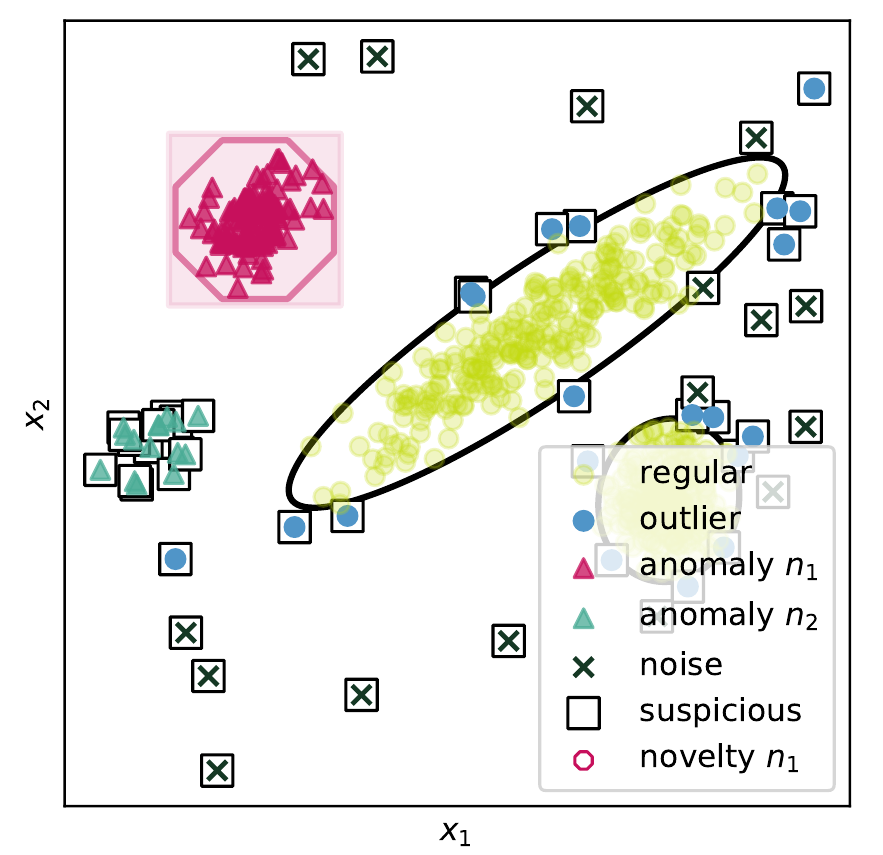
\includegraphics[width=0.8\textwidth]{images/gruhl_anomaly_definition.png}
  \caption{Classification of diefferent anomalies \cite[p. 54]{gruhl_novelty_2022}}
  \label{fig_anomaly_gruhl}
\end{figure}

% definiton by shape
Instead of dividing anomalies by their cause the shape of anomalies can vary in several ways. In real measurement data any shape is possible and it is totally unpredictable \cite{schwartz_maeday_2024}. For training purposes anomaly injection is crucial. Then the anomalies are simulated as point anomalies or subsequence anomalies. Point anomalies occur once and can be global or contextual. Subsequence anomalies on the other hand change the values in a given time window or on long term. They can be divided in seasonal, shapelet and trend anomalies. Seasonal and shapelet anomalies change the values in a limited time window, trend anomalies are changing all following values \cite[p. 9]{darban_carla_2024}. %Seasonal in time direction, shapelet the amplitudes

% definiton for this paper
In this paper we want to focus on single time events, which are in any case anomalies. Potentially being caused by an unknown process, they cannot be classified \cite{gruhl_novelty_2022}. This defines our goal as an Anomaly Detection (AD) task.

\subsection{Zero Shot Learning}
%Definiton by Chandana
In this paper the definition made by \cite{nivarthi_unified_2022} is used. They seperate Single Task Learning, where every model is trained seperately for each task, from Multi Task Learning (MTL) where one model is trained and evaluated on several tasks. For Zero Shot Learning (ZSL) in comparison the model is trained on several tasks like in MTL but tested on completely new ones.

% Zero Shot derived from Transfer learning
Zero Shot Learning is therefore an extreme form of transfer learning. While transfer learning is the concept of transferring the knowledge and weights gained at one task using them at solving another task, Zero-Shot Learning means there are no samples for the other task. The transformation of knowledge can help solving tasks where there are few or no samples available. The gained knowledge is normally stored as representations in data. Representations which are abstract enough to not see a specific item but information about items. This also means that ZSL is only possible because additional information has been discovered during training \cite[p. 536]{goodfellow_deep_2016}.

% First zero shot detection
\cite{palatucci_zero-shot_2009} were the first to implement a successful Zero-Shot Detection followed by \cite{socher_zero-shot_2013} who used semantic word vector representations to classify words in groups and to sort new words with an accuracy of 90\% with a fully unsupervised model.

Zero-shot learning involves training a model on certain classes and then testing its ability to recognize new, unseen classes without any retraining. In the context of anomaly detection, this means the model should be able to detect types of anomalies it has not encountered during the training phase.

\section{Representation Learning Methods}\label{review}
In this chapter any found paper proposing a RL strategy used for time series data with adaptability on anomaly detection tasks is presented. For the literature research the inclusion criteria as described in \ref{criteria} are applied.

The different RL strategies explained focusing on the compliance of the exclusion criteria. The strategies are organized by their underlying concept. We begin with straight-forward methods which are based on one concept and increase the complexity throughout the chapter. In the end methods that use combinations of different concepts are presented.
\subsubsection{MLP}
% INRAD
Using a simple MLP is a straight-forward way to learn representations and to detect anomalies in time series data \cite{nielsen_neural_2015}. The input variable for the MLP are time points and the output variable represents the value at these time points. The model is trained to learn this mapping. With the trained model, the values in a live scenario are predicted and the difference to the actual values is measured. If the difference exceeds a certain threshold, an anomaly is found. A method called INRAD, Implicit Neural Representation of Time-Series Data is using this concept. The method takes multiple variables as input and the model is trained with data including anomalies. It is not suitable for Zero-Shot Learning \cite{jeong_time-series_2022}.
\subsubsection{RNN}
\cite{su_robust_2019} propose a method called OmniAnomaly for anomaly detection in multivariate time series data using a Stochastic Recurrent Neural Network (SRNN). This approach addresses the challenge of detecting anomalies in complex, high-dimensional time series data.
Their method utilizes a SRNN to model the temporal dependencies in multivariate time series data.
The key advantage of this method is its robustness to noisy and high-dimensional data. The SRNN learns to represent the normal patterns in the time series and identifies deviations from these patterns as anomalies. It relies on training with data that contains normal patterns, which the model uses to detect anomalies based on deviations from these patterns. Since OmniAnomaly depends on having access to representative normal data to learn patterns, it is not suitable for zero-shot scenarios.
\subsubsection{CNN}
Methods based on Convolutional Neural Networks (CNN) are normally used to classify images but in recent papers they are used to detect anomalies in images. \cite{aota_zero-shot_2023} develop a Texture Anomaly Detection and achieve a high performance in Zero Shot Learning. They compare Zero-Shot against Many-Shot Learning in their work. Several image anomaly detection tools can be found (\cite{sabokrou_deep-anomaly__2018}, \cite{aota_zero-shot_2023}). But CNNs perform on time series data as well.

The main idea of using CNNs is to predict a value based on the input frame. If the distance between the predicted and the actual value exceeds a predefined threshold, the anomaly can be detected.

% CyberAttacks Kravchick
This idea is used to detect cyberattacks in industrial control systems. The study by \cite{kravchik_detecting_2018} uses a dataset from a Secure Water Treatment testbed to identify cyber anomalies by measuring the statistical deviation between predicted and observed values. They explore different deep learning architectures, including CNNs and recurrent networks, and find that 1D CNNs perform particularly well for time series prediction tasks. Their approach successfully detects the majority of cyber attacks with minimal false positives, highlighting the effectiveness of CNNs in real-time anomaly detection in multivariate time series \cite{kravchik_detecting_2018}. However, the paper does not discuss the usability on zero-shot learning. In the same area a method detecting unknown cyber-attacks is presented by \cite{zhang_unknown_2020} who use an Autoencoder which is discussed later on.

% TCN
\cite{he_temporal_2019} use Temporal Convolutional Networks (TCN). TCNs restrict the output to be dependent on past and present time steps only. This enables them to capture temporal dependencies. By training on normal patterns, the network learns to predict future values. Significant deviations between these predictions and actual observations indicate potential anomalies. Since the model only learns the normal data, it is able to work in Zero Shot scenarios. The inclusion of a multivariate Gaussian model for error handling and the multi-scale feature mixture method enhances the robustness and accuracy of the anomaly detection process.

% SLMR
Another paper introduces a mask-based self-supervised representation learning approach to extract both short-term local dependencies and long-term global trends. By integrating forecasting and reconstruction-based models, the method effectively captures temporal contexts and feature correlations. An attention mechanism ensures feature importance, leading to better anomaly detection performance on various datasets. The method is designed for multivariate time series anomaly detection but does not explicitly address zero-shot learning scenarios.
\cite{miao_unsupervised_2022}

\subsubsection{Contrastive Learning}
% Paper Debiased Contrastive Learning
Learning representations in time series data is done in several different ways. One solution according to \cite{zhang_debiased_2024} is contrastive learning. By comparing pairs of data points and rating the similarities as distances between the two, CL gets less dependent on labeled data. The data can be more general and the extracted representations are more robust. The pairs of data points are labeled as positive and negative pairs with a distance according to their similarities. With this distance they are put into a feature space where they form groups of data points. To minimize the bias between representations, multigranularity augmented view generation and expert knowledge are used during training. The proposed framework is applied on industrial fault detection. The two data sets consist of various vibration signals of industrial machines and stiction sensors with multiple variables. The effectiveness of the proposed framework is demonstrated through its application to these datasets.

% CARLA
CL is also used for anomaly detection in time series data by \cite{darban_carla_2024}. They use CL combined with synthetic anomaly injection. CL enables them to capture patterns in time series data and the framework shows good results on common real world datasets. Like in the previous paper, dissimilar pairs, the anomalies, build distant data points and similar data points are close to each other. In order to train the model artificial anomalies are injected which build distant pairs. In the next stage the classification is done by  the proximity of the neighbours in the representation space. Additionally anchor points representing the nearest and furthest neighbour are given from each representation. Their methodology is called CARLA and is not tested for Zero-Shot Learning. An implementation by the authors can be found \footnote{\fussy\tiny github.com/zamanzadeh/CARLA}.

% CL-TAD
CL-TAD, a method for time series anomaly detection that leverages contrastive learning and reconstruction-based techniques addresses the challenges of temporal dynamics, label scarcity, and data diversity in real-world applications. The method comprises two main components: positive sample generation and contrastive-learning-based representation learning. Positive samples are generated by reconstructing masked parts of the time series data, helping the model learn the underlying normal patterns. These samples, along with the original data, are then fed into a contrastive learning framework, which contrasts pairs of similar and dissimilar samples to learn representations. This process helps the model map similar data points closer together in the feature space while distancing dissimilar points, making it easier to detect deviations indicative of anomalies \cite{ngu_cl-tad_2023}.
While CL-TAD is not explicitly designed as a zero-shot learning method, its use of contrastive learning and reconstruction-based techniques suggests that it could have potential in zero-shot anomaly detection scenarios. A tutorial for implementation can be found \footnote{\fussy\tiny github.com/nguhcv/cl-tad/tree/main}.

% OCC based methods
% COCA
To succeed on Zero-Shot Anomaly Detection, One-Class Classification (OCC) can be useful.
By gathering all "normal" values into a single class the outliers are directly detected if they are outside of it.
The COCA (Contrastive One-Class Anomaly Detection) method combines contrastive learning with OCC to improve anomaly detection in multivariate time-series data. By treating original and reconstructed representations as positive pairs, it optimizes a contrastive one-class loss function that enhances the detection of anomalies while preventing common issues like hypersphere collapse. Although COCA is designed for self-supervised anomaly detection, its ability to learn from unlabeled data suggests potential applicability in zero-shot learning scenarios, though this has not been explicitly tested \cite{wang_deep_2023}. An implementation script is provided by the authors \footnote{\fussy\tiny github.com/ruiking04/COCA}.

%
The paper by \cite{lee_time_2023} presents an approach for detecting anomalies also using OCC in industrial time series data, which typically lacks labels for supervised learning. They combine OCC with contrastive learning to define a new objective function that can simultaneously learn from both models. This method enhances feature extraction while preserving temporal characteristics. The paper demonstrates the method's effectiveness through high anomaly detection performance on datasets with similar normal and anomalous data forms, highlighting its potential in industrial applications.

Unlike traditional OCC methods that map all normal instances into a single hypersphere, the method presented by \cite{chen_time-series_2023} focuses on local contextual information. By pulling each normal instance towards its recent context window, it aims to better detect context-based anomalies. The model incorporates a deterministic contrastive loss, which improves the network's ability to distinguish between normal and abnormal data.

% TS2Vec
\cite{yue_ts2vec_2022} introduce TS2Vec, a framework for learning robust and universal time series representations at multiple semantic levels through hierarchical contrastive learning. This approach utilizes timestamp masking and random cropping to create augmented context views, enhancing position-agnostic and comprehensive representations. By combining instance-wise and temporal contrastive losses, TS2Vec captures characteristics of different time series instances and dynamic temporal patterns within each series. The method is tested on Zero Shot Learning and is applicable for multivariate time series data. The instructions on reproducing the outcomes are made publicly available by the authors \footnote{\fussy\tiny github.com/zhihanyue/ts2vec \label{foot_ts2vec}}.

% TimeAutoAD
Another paper introduces an autonomous system for anomaly detection in multivariate time series data also using Contrastive Learning. The proposed TimeAutoAD automates model configuration and hyperparameter optimization, addressing challenges such as limited labeled anomaly data. It uses self-supervised contrastive learning to enhance the model's ability to differentiate normal and anomalous time series by generating pseudo-negative samples. The method is tested on real-world datasets, demonstrating improved performance over existing anomaly detection techniques, especially in scenarios where training data may be contaminated. The paper does not explicitly address zero-shot anomaly detection \cite{jiao_timeautoad_2022}.

% ContrastAD
The ContrastAD framework presented in \cite{li_contrastive_2023} is a self-supervised method for time series anomaly detection that leverages contrastive learning with temporal transformations. The key innovation is the use of anomaly-induced transformations to create representations that differentiate between normal and abnormal data. This approach targets both point anomalies and contextual anomalies in high-dimensional time series, which are often missed by other methods. By learning distinct representations for normal and anomalous data in the latent space, ContrastAD improves performance on noisy and complex datasets. However, the method is not trained or validated on entirely new types of anomalies.

% DCdetector
Another model called DCdetector presented in \cite{yang_dcdetector_2023} is a multi-scale dual attention contrastive learning framework designed for time-series anomaly detection. It utilizes a dual attention asymmetric design to create a permutation-invariant representation, guiding the learning process with pure contrastive loss. This approach enhances the model's ability to discriminate between normal and anomalous data. Extensive experiments demonstrate that DCdetector achieves state-of-the-art performance across multiple benchmark datasets. While the paper focuses on its effectiveness in anomaly detection, it does not explicitly address or test the model's applicability to zero-shot learning scenarios \cite{yang_dcdetector_2023} In the article a repository containing bash scripts for implementation can be found \footnote{\fussy\tiny github.com/DAMO-DI-ML/KDD2023-DCdetector}.

%Contrastive Predictive Coding Methods:
\cite{pranavan_contrastive_2022} presents a novel approach for anomaly detection in multi-variate time series data using Contrastive Predictive Coding (CPC). Their method, named Time-series Representational Learning through Contrastive Predictive Coding (TRL-CPC), aims to capture the temporal dependencies and correlations across multiple variables in time series data.
The TRL-CPC framework consists of an encoder, an auto-regressive model, and a non-linear transformation model. These components are optimized to learn the representations of multi-variate time series data by predicting future segments from past segments. The core idea is to maximize the mutual information between the encoded representations of past and future segments, thereby learning robust representations.
To detect anomalies, TRL-CPC calculates the prediction error between actual future segments and the predicted segments generated by the CPC model. Anomalies are identified where this prediction error exceeds a certain threshold, enabling unsupervised anomaly detection based on the structure of the data itself \cite{pranavan_contrastive_2022}.

% TiCTok
CPC is also used by the method TiCTok presented in \cite{kang_tictok_2023}. The model proposes an approach to multivariate time-series anomaly detection by combining contrastive tokenization with a time-series token encoder. This encoder converts raw time-series data into latent embeddings that capture wide-ranging temporal information. The model employs contrastive learning to produce representations, which help distinguish between normal and anomalous data. Additionally, TiCTok introduces a new anomaly scoring method based on the contrastive loss used during training. In their paper they do not test the model on Zero Shot Learning scenarios.

% MGCLAD
Another paper introduces Multiview Graph Contrastive Learning for detecting anomalies in multivariate time-series data, particularly in IoT systems. The method constructs graph structures to model both temporal context and signal dependencies, while an adaptive data augmentation strategy generates graph views for contrastive learning. This approach enhances representation quality and improves performance in anomaly detection tasks except Zero Shot Learning \cite{qin_multiview_2023}. The method is available on Github \footnote{\fussy\tiny github.com/shuxin-qin/MGCLAD}.

% TriAD
The paper by \cite{sun_unraveling_2023} introduces TriAD (Tri-domain Anomaly Detector), a self-supervised learning method for time-series anomaly detection. TriAD models features across three domains: temporal, frequency, and residual. Without relying on labeled anomalies. Unlike traditional contrastive learning, TriAD uses inter-domain and intra-domain contrastive losses to learn shared attributes among normal data and distinguish them from anomalies. The approach is designed to handle anomalies of varying lengths and shapes \cite{sun_unraveling_2023}. The authors provide a link to their implementation \footnote{\fussy\tiny github.com/pseudo-Skye/TriAD}.

In summary methods using contrastive learning are mostly not tested on Zero-Shot Learning. Their robustness against noisy data is not ensured.

\subsubsection{Autoencoder}
Autoencoders on the other hand are robust to unclean training datasets \cite[p. 2487]{abdulaal_practical_2021}. Due to their architecture noise is filtered from the input.

\cite{provotar_unsupervised_2019} introduces an anomaly detection method using an autoencoder architecture based on Long Short-Term Memory (LSTM) networks. The core idea is that an LSTM autoencoder learns to compress and reconstruct the input time series data. During training, the model learns the normal patterns in the data by minimizing the reconstruction error. When fed new data, the model attempts to reconstruct it, and any significant reconstruction error (i.e. deviation between the original and reconstructed data) signals an anomaly. This approach is particularly effective because LSTMs are well-suited to capture temporal dependencies, making them ideal for time series data. The model works without requiring labeled datasets, making it an unsupervised solution. The authors test the model on both synthetic and real-world data, such as sound event detection. It can effectively detect outliers based on reconstruction error but does not have the capacity for ZSL.

% TSMAE
Time Series Memory-Augmented Autoencoder (TSMAE), a anomaly detection method for IoT time-series data integrates a memory module to suppress overgeneralization by storing normal patterns and reconstructing time-series data with Long Short-Term Memory (LSTM) networks to capture temporal dependencies. Anomalies are detected by comparing the reconstruction error between the original and generated sequences, enhancing anomaly detection effectiveness. This method is tested on multivariate time series data, but no explicit mention of zero-shot testing was found \cite{gao_tsmae_2023}.

%UAE-TENN
\cite{nivarthi_multi-task_2023} are the first to use a Unified Autoencoder (UAE) for time series data, namely the power forecast of wind and solar plants. They contribute to the challenge of predicting the possible outcome of renewable energy in a newly created plant, either wind or solar. To do so a UAE is combined with a Task Embedding Neural Network (TENN). They examine the usability divided in Single-Task, Multi-Task and Zero-Shot Learning. The method was first published in \cite{nivarthi_unified_2022}. It is then extended by convolutional layers instead of the fully connected neural network layers (UCAE-TENN) and also Long Short-Term Memory layers (ULAE-TENN).

% MST-VAE
\cite{pham_mst-vae_2022} proposes a Multi-Scale Temporal Variational Autoencoder (MST-VAE) for anomaly detection in multivariate time series data. MST-VAE combines short and long-scale convolutional kernels within a 1D CNN and a Variational Autoencoder to capture both short-term and long-term temporal patterns. The method is not directly tested in a Zero-Shot scenario. An implemention is provided by the authors \footnote{\fussy\tiny github.com/tuananhphamds/MST-VAE}.

% MSCVAE
Another method using VAE introduces a Multi-Scale Convolutional Variational Autoencoder (MSCVAE) for unsupervised anomaly detection in multivariate time-series data. It constructs multi-scale attribute matrices to capture system states at different time steps and uses a convolutional variational autoencoder to extract spatial features, while an attention-based ConvLSTM captures temporal patterns. Anomalies are detected by comparing the original and reconstructed matrices, and a novel ERR-based threshold strategy is employed for optimal performance. The article does not mention Zero-Shot Learning and neither provides an open source implementation \cite{yookampon_robust_2022}.

% VRAE based
To detect anomalies in healthcare data a variational recurrent autoencoder (VRAE) is used in \cite{pereira_learning_2019}. They created an unsupervised framework where the model learns to represent the data and detect anomalies without needing labeled examples.
The model works by learning to reconstruct the input sequences. During training, they add noise to the input data, and the model tries to reconstruct the original, uncorrupted data. This helps the model learn more robust representations of the data. To detect anomalies, they cluster these learned representations and calculate the distance to identify outliers. Their approach was tested on the ECG5000 dataset and showed that it could effectively detect unusual heartbeats, performing better than previous methods that required labeled data. The model is designed to capture temporal dependencies, making it applicable for MVTSD.

%
Another approach using VRAE involves creating synthetic anomalies to improve the detection process. A two-level hierarchical latent space representation is used. First, they distill feature descriptors of normal data points into more robust representations using AEs. These representations are then refined using a VAE that creates a family of distributions. From these distributions, they select those that lie on the outskirts of the normal data as generators of synthetic anomalies.
By generating these synthetic anomalies, they train binary classifiers to distinguish between normal and abnormal data. Their hierarchical structure for feature distillation and fusion helps create robust representations, enabling effective anomaly detection without needing actual anomalies during training \cite{ramirez_rivera_anomaly_2022}.

% VRQRAE
Kieu et al. propose Variational Quasi-Recurrent Autoencoders (VQRAEs) for unsupervised time series anomaly detection, using robust divergences to improve resilience against noisy data. VQRAEs utilize Quasi-Recurrent Neural Networks (QRNNs) for efficient temporal dependency capture, and a bi-directional version (BiVQRAEs) enhances accuracy by processing data in both forward and backward directions. However the method was not explicitly tested on Zero-Shot Learning \cite{kieu_anomaly_2022} \footnote{\fussy\tiny github.com/tungk/Bi-VQRAE}.


% Unknwon CyberAttacks
The paper by \cite{zhang_unknown_2020} addresses the challenge of detecting unknown cyberattacks by applying zero-shot learning. The proposed method maps the features of known attacks to a semantic space using a sparse autoencoder and restores them to the feature space by minimizing reconstruction errors, effectively creating a mapping between features and semantic attributes. This technique enables the model to detect previously unseen attacks by generalizing from known attack features. The research highlights the feasibility and effectiveness of zero-shot learning for cybersecurity applications.

% FuSAGNet
A method called Fused Sparse Autoencoder and Graph Net (FuSAGNet) is used for anomaly detection in multivariate time series data, specifically targeting cyber-physical systems. The method combines a Sparse Autoencoder (SAE) to learn sparse latent representations and a Graph Neural Network (GNN) to forecast future time series behavior. It captures both temporal dependencies and complex inter-feature relationships by learning graph structures from the data. This joint optimization approach aims to improve anomaly detection performance by fusing reconstruction and forecasting tasks. The method was empirically tested on three real-world datasets related to industrial systems but not in Zero-Shot Learning scenarios \cite{han_learning_2022} \footnote{\fussy\tiny github.com/sihohan/FuSAGNet}.

% deep AOC
Deep Autoencoding One-Class (AOC), a method for time-series anomaly detection that combines autoencoder-based reconstruction and one-class classification in a single-stage approach to better capture normal patterns. The method is evaluated on public datasets, outperforming baseline models and proving effective for detecting various types of anomalies in both univariate and multivariate time-series data. However, zero-shot learning is not tested or addressed in the proposed framework \cite{mou_deep_2023} \footnote{\fussy\tiny github.com/alsike22/AOC}.

% RANSynCoders
Another paper presents a method named RANSynCoders for detecting anomalies in asynchronous multivariate time series by combining spectral analysis with autoencoders. It leverages spectral analysis to synchronize the features, followed by multiple autoencoders using random feature subsets to detect anomalies via majority voting. This approach improves performance on high-dimensional, asynchronous data by reducing false positives and providing better localization of anomalies. The method in the paper does not specifically mention being tested in zero-shot scenarios \cite{abdulaal_practical_2021}. An implemention of the method is provided by the authors \footnote{\fussy\tiny github.com/eBay/RANSynCoders}.

% TCN-AE
Another proposed method is using a Temporal Convolutional Network Autoencoder (TCN-AE) designed for unsupervised anomaly detection in multivariate time series data. It employs dilated convolutions to capture long-range dependencies and compresses time series into representations using an autoencoder. The method detects anomalies by evaluating reconstruction errors, as anomalies are expected to have significantly higher reconstruction errors compared to normal patterns \cite{thill_temporal_2021}. A Repository with a minimal working example can be found provided by the author but no implementation on new datasets is provided \footnote{\fussy\tiny github.com/MarkusThill/bioma-tcn-ae}.



% MEGA
A framework called Multiscale Wavelet Graph AutoEncoder (MEGA) presented in \cite{wang_multiscale_2023} for anomaly detection in multivariate time series. It integrates Discrete Wavelet Transform (DWT) to decompose time series into different frequency components, reconstructing them to highlight anomalies across scales. Additionally, a dynamic graph convolution network is employed to model inter-variable relationships at different scales, enhancing the detection of anomalies caused by changes in variable dependencies.
This method is tested in a zero-shot scenario and explicitly takes multivariate time series as input. The code can be found provided by the authors \footnote{\fussy\tiny github.com/jingwang2020/MEGA}.

% DAEMON
The method proposed in \cite{chen_adversarial_2023} introduces DAEMON, an adversarial autoencoder framework designed for unsupervised multivariate time-series anomaly detection and interpretation. The model employs two adversarial training processes: one to align the hidden variable’s posterior distribution with a prior and another to minimize the difference between original and reconstructed data. This improves robustness and avoids overfitting while anomalies are detected based on reconstruction errors. There is no mentioning of testing in a zero-shot scenario.
Replicating the results of the paper is possible due to the open source availability mentioned in the paper
\footnote{\fussy\tiny github.com/Sherlock-C/DAEMON \label{foot_daemon}}.


% GRU-AE
The method proposed in \cite{gong_autoencoder-based_2022} utilizes a Gated Recurrent Unit-based Autoencoder (GRU-AE) to detect anomalies in time-series data by reconstructing sequences and identifying large reconstruction errors as anomalies. It incorporates an attention mechanism to enhance performance and applies multi-timestamp stacking to reduce time steps for better training efficiency. The model is tested on real-world datasets from cellular networks, detecting anomalies at both single-day and multi-day scales. The method is applied to multivariate time-series data, but no mention of a zero-shot scenario is made.

%
The method proposed in \cite{wang_attention-based_2022} presents an attention-based encoder-decoder network for anomaly detection in time-series data, which focuses on learning representations in both principal and residual spaces without needing reconstruction. The attention mechanism is applied to rescale convolutional layers, highlighting the most contributive segments of the data for better representation learning. This approach improves anomaly detection by calculating belief scores in both spaces using kernel density estimation (KDE). The method is tested on multivariate time series and in a zero-shot scenario, specifically for detecting new faults.

% MOMENT
To overcome the challenge of poorly available time series data sets \cite{ma_survey_2023}, the model family MOMENT tries to learn general patterns on a pile of time series data. The pile is a collection of different datasets which they assembled for their pretraining. According to the paper minimal finetuning is needed to perform on multivariate time series tasks like anomaly detection. They published the model and made the usage easily accessible with its own python library. The time serie datasets the model is trained on consist of domains including weather measurements, sensor values and power consumption datasets. They also included tongue and finger movement of humans. The different tasks which the model is evaluated on are forecasting (long and short horizon), classification, anomaly detection and imputation. Except for short-horizon forecasting all tasks are managed well. However it cannot detect anomalies in vertically shifted time series \cite{goswami_moment_2024}. The method is available as a Jupyter Notebook on Github \footnote{\fussy\tiny github.com/moment-timeseries-foundation-model/moment/blob/main/tutorials/anomaly\_detection.ipynb \label{foot_moment}}.

% \cite{zhang_debiased_2024} point out, that AE-based methods have remaining challenges.
% TODO what are the challenges of autoencoders?

\subsubsection{Transformer}
% AnomalyTransformer
\cite{xu_anomaly_2022} use a Transformer architecture to detect anomalies on three different datasets. \footnote{\fussy\tiny github.com/thuml/Anomaly-Transformer}

%TranAD
\cite{tuli_tranad_2022}
\footnote{\fussy\tiny github.com/imperial-quore/TranAD}

% DATN TODO
\cite{wu_decompose_2023}

% TiSAT TODO
\cite{doshi_tisat_2022}

% TCF-Trans TODO
\cite{peng_tcf-trans_2023}

% DCT-GAN TODO
\cite{li_dct-gan_2023}

% GRU-AE TODO
\cite{shin_time_2023}


% LLMs
Based on the transformer architecture, Large Language Models (LLM) are developed and used increasingly in different applications. Known as chatbots they can help in language specific tasks. Beside that they can be used in anomaly detection and forecasting. \cite{su_large_2024} examine a literature review on how LLMs perform on anomaly detection tasks concerning time series data. LLMs in anomaly detection are specifically useful when the time series data is in the form of words. This can be the case in log analysis. Logs are generated over time and hold a lot of information which can singify errors and system failures. They conclude that LLMs have potential in detecting anomalies but challenges remain. The occurrence of hallucinations and the need for computational efficiency to name a few.

A method detecting anomalies in tabular data using LLMs is presented by \cite{li_anomaly_2024}. In order to perform tasks that LLMs are not directly build for they generate synthetic datasets. Using these datasets LLMs and specifically GPT-4 have comparable performance with transductive learning methods \cite[p. 6]{li_anomaly_2024}.

% Fourier
Using Fourier Analysis and the transformer architecture \cite{ye_multivariate_2023} detect anomalies in time series data. The encoder of a transformer is used to capture temporal features of time series. They detect frequencies by using Fourier Analysis.

\subsubsection{Shapelet Learning}
% Shapelets: Shapelets are short, representative subsequences extracted from time series data.
% Shapelet Learning: Extraction, Evaluation and Selection of shapelets. Medling
\cite{beggel_time_2019} address the problem of detecting anomalies in time series data using a novel unsupervised method based on shapelet learning. This approach is particularly useful in scenarios where labeling data is difficult and expensive.
Their method learns representative features that describe the shape of time series data from the normal class and simultaneously learns to accurately detect anomalies. The objective function encourages the learning of a feature representation in which normal time series lie within a compact hypersphere, while anomalous observations lie outside the decision boundary. This is achieved through a block-coordinate descent procedure.
The advantage of their approach is that it can efficiently detect anomalies in unseen test data without retraining the model, by reusing the learned feature representation. Experimental results on multiple benchmark datasets demonstrate the robustness and reliability of the method in detecting anomalous time series, outperforming competing methods when the training data contains anomalies.

% Alshaer
In contrast, \cite{alshaer_detecting_2020} propose a method combining matrix profiles with shapelet learning to handle streaming time series data. The matrix profile efficiently identifies potential anomalies in real-time, and shapelet learning characterizes these anomalies accurately. This approach is particularly suited for environments requiring immediate anomaly detection, such as finance, healthcare, and industrial monitoring.

% shapelet summary
While both methods utilize shapelet learning, Beggel et al. focus on static datasets and robust feature representation, whereas Alshaer et al. emphasize real-time detection in dynamic, streaming environments.
% TODO search for GAN based methods

% SL based TODO
\cite{liang_shapelet-based_2024}

% IPS TODO
\cite{li_ips_2022}

\subsubsection{Other}
% Clustering
\cite{li_clustering-based_2021} propose a method for detecting anomalies in multivariate time series by combining clustering and reconstruction techniques. The authors use a sliding window approach to generate subsequences from the multivariate time series, then apply extended fuzzy clustering to reveal the underlying structure of the subsequences. By reconstructing these subsequences with optimal cluster centers, the method detects anomalies based on how well the reconstructed data fits the original subsequences. A confidence index quantifies the level of detected anomalies. The approach is shown to effectively detect anomalies related to amplitude and shape changes in various application domains, such as healthcare and finance, and is optimized using Particle Swarm Optimization.

% TODO include benchmark methods from \cite[p. 19]{darban_carla_2024}

% LSTM based TODO
\cite{niu_lstm-based_2020}
% Moving Memory Dynamic Filter TODO
\cite{duan_unsupervised_2021}

\section{Application for Zero Shot Anomaly Detection on Multi Variate Time Series Data}\label{application}
In this chapter the found articles are filtered using the exclusion criteria defined in chapter \ref{criteria}. By excluding methods that haven't been tested with multiple input variables we answer RQ2. Methods that are not tested in Zero-Shot Learning Scenarios are also excluded which covers RQ4.

More precisely we want to know by the defined filter process which of the proposed RL types are best suited for Zero Shot Anomaly Detection in multi-variate time series data. In this chapter a selection of appropriate methods for Time Series Data Anomaly Detection out of \ref{review} is extracted.

% TODO table like in gruhl
 % table
 In order to achieve a successful implementation in the following chapter only models which are available and well documented are chosen for further examination. Representation learning methodologies matching the inclusion criteria and their classification by exclusion criteria are listed in table \ref{tab_rl_methods}
 \begin{table}
   \caption{Abbreviations: Transformer (T), Clustering (C), multiple input variables (MV), open source availability (OSA). Legend: yes: \cmark, no: \xmark, no information: -.}\label{tab_rl_methods}
   \begin{longtable}[]{@{}llllll@{}}
\toprule\noalign{}
Method Name & Author & Concept & MV & ZSL & OSA \\
\midrule\noalign{}
\endhead
\bottomrule\noalign{}
\endlastfoot
INRAD & Jeong et al. & MLP & & \xmark & \cmark \\
OmniAnomaly & Su et al. & RNN & & \xmark & \cmark \\
CNN based method & Kravchik et al. & CNN & & \xmark & \\
CNN based method & He et al. & CNN & & \xmark & \xmark \\
CL based method & Zhang et al. & CL & & \cmark & \xmark \\
CARLA & Darban et al. & CL & & \xmark & \\
CL-TAD & Ngu et al. & CL & & \cmark & \\
COCA & Wang et al. & CL & & \xmark & \\
CL based method & Lee et al. & CL & & & \\
CL based method & Chen et al. & CL & & \xmark & \\
TS2Vec & Yue et al. & CL & \cmark & \cmark & \cmark \\
TimeAutoAD & Jiao et al. & CL & & \xmark & \\
ContrastAD & Li et al. & CL & & \xmark & \\
Dcdetector & Yang et al. & CL & & \xmark & \\
TRL-CPC & Pranavan et al. & CL & & \xmark & \\
TiCTok & Kang et al. & CL & & \xmark & \\
MGCLAD & Qin et al. & CL & & \xmark & \\
TriAD & Sun & CL & & \xmark & \\
UCAE-TENN & Nivarthi et al. & AE & & & \\
MAEDAY & Schwartz et al. & AE & & & \\
VRAE based method & Pereira et al. & AE & \cmark & \cmark & \xmark \\
AE based method & Ramirez et al. & AE & & & \\
AE based method & Provotar et al. & AE & \cmark & \xmark & \xmark \\
FuSAGNet & Han et al. & AE, GNN & \cmark & & \\
MSTVAE & Pham et al. & AE & \cmark & & \\
deep AOC & Mou et al. & AE & & & \\
AE based method & Zhang et al. & AE & & \cmark & \\
RANSynCoders & Abdulaal et al. & AE & & & \cmark \\
VRQRAE & Kieu et al. & AE & & & \xmark \\
TCN-AE & Thill et al. & AE & & & \\
MEGA & Wang et al. & AE & \cmark & & \\
DAEMON & Chen et al. & AE & \cmark & \cmark & \xmark \\
TSMAE & Gao et al. & AE & & & \\
GRU-AE & Gong et al. & AE & & & \\
MSCVAE & Yokkampon et al. & AE & \cmark & \cmark & \\
MOMENT & Goswami et al. & T & & \cmark & \cmark \\
TranAD & Tuli et al. & T & & & \cmark \\
Transformer based method & Ye et al. & T & & & \\
AnomalyTransformer & Xu et al. & T & & & \cmark \\
DATN & Wu et al. & T & & & \\
LLM based method & Li et al. & T & & & \\
TiSAT & Doshi et al. & T & & & \\
TCF-Trans & Peng et al. & T & & & \\
DCT-GAN & Li et al. & T & & & \\
& Li et al. & C & & & \\
& Beggel et al. & SL & & & \\
& Alshaer et al. & SL & & & \\
& Aota et al. & & & & \\
& Niu et al. & LSTM & & & \\
\end{longtable}

 \end{table}

\section{Proof of Concept}\label{implementation}
The best fitting strategies extracted in \autoref{application} are implemented on a small test data set in order to demonstrate how and if they work. First the used dataset ant the purpose of anomaly detection for the specific use case is described. Later the process of implemention and the results are presented.
\subsection{Inverter data including Anomalies}
While NLP and image processing tasks are common and a variety of data sets exists, time series data sets are not available that much \cite{ma_survey_2023}. Thanks to the employees of SMA a multivariate time series dataset is provided. The specific use case and the structure of the chosen data is described in this section.

% Use case for sma
SMA developes and manufactures inverters for home and commercial use. The inverters convert direct to alternating current or vice versa depending on the use case. They also act as home managers controlling all energy flows in a power plant. Inverters are equipped with several sensors measuring the surroundings and internal states in order to maximize the efficency and to avoid system failures. Sometimes system failures appear still which raises the question if this could have been foreseen by analyzing the gathered sensor data during runtime. The first step to reach such a forecasting tool is to detect the anomalies in recorded sensor data. The implementation of the chosen methods is therefore done on inverter data provided by the company.

% Features in data
The variables contain measurements of current and voltage of all phases in AC and the generated DC sources. Additionally temperatures, CPU usage, internal parameter settings and many other measurements are included. The total number of features is 137.

% Data structure
The values are collectively stored at a 7 minute interval over several months. 19 inverters that had system failures at some point are taken into account. These failure time stamps are known and added as an additional feature with a binary value of 1. Every other error bit is 0. The data is collected between 2018 and 2020 and the locations of the inverters cannot be provided.

% TODO DEfiniton of training and test data
% In the test data the learning data is seperate from the data including anomalies. The important thing about Zero Shot Learning is that a specific anomaly never occured like this before. In the test data, all chosen representation learning techniques are applied using the same data for learning and afterwards testing the anomaly detection with the same anomalies. According to chapter (Evaluation) the characteristics are evaluated for each RL technique chosen in the previous chapter.

\subsection{Implemented Methods}
The main goal is to detect the labeled anomalies in the SMA dataset. If the methods find the timestamp of the system failure, they perform correctly. First the models are taken as is and a forward pass is applied. The given output is evaluated if the model already detects the failure time points in the inverter time series data. If possible, the model is trained afterwards using a set of 12 inverters and tested on the remaining 7 inverters. This way the Zero-Shot scenario like in \autoref{theory} is created.
The code for the implementions can be found on link \footnote{\fussy\tiny github.com/johanneshoelker/Smart-Systems-Paper/tree/main/Implementation}.

%Carla
\subsubsection{CARLA}
An implemention of the model CARLA is done by the authors using Python available on \autoref{foot_carla}. The repository contains scripts for replicating the results, but no further information on how to adapt the model on new datasets is given.

% TS2Vec
\subsubsection{TS2Vec}
An implemention of the model TS2Vec is done by the authors using Python which is available on \autoref{foot_ts2vec}. A function for preprocessing the data to fit as an input for the model was written.
Using the function a successful forward pass was made. The learned representations can be used for further evaluation.

% MEGA
\subsubsection{MEGA}
According to \cite{wang_multiscale_2023} the model MEGA is trained and evaluated on three different datasets. The code for reproduction is provided by the authors. They implement the model using Python on \autoref{foot_mega}. No further information on how to adapt the model on new datasets is given but the scripts are adapted to run successfully with SMA data as multivariate input. The output was not further reviewed.

\subsubsection{DAEMON}
The authors of the method DAEMON published python scripts for replicating the results on all datasets they used \cite{chen_adversarial_2023}. However, no explanation on how to use the method for entirely new datasets can be found on this \autoref{foot_daemon}.

% Moment
\subsubsection{MOMENT}
A detailed instruction on how to reproduce the outcomes of MOMENT presented by \cite{goswami_moment_2024} is provided on this GitHub \autoref{foot_moment}. The method takes a three dimensional input tensor, containing batches, channels and time points. The maximal number of points is 512. It reconstructs the given input and returns a tensor containing the reconstructions.

For the implementation on SMA data the provided tutorial is used as a guide. The SMA data is preprocessed to match the requested input tensor. The reconstructions are further compared with the inputs by calulating the Mean Squared Error (MSE):
\begin{equation}
    \text{MSE} = \frac{1}{n} \sum_{i=1}^{n} \left( y_i - \hat{y}_i \right)^2
\end{equation}
The error is further normalized using the Min-Max Normalization:
\begin{equation}
x' = \frac{x - \text{min}(x)}{\text{max}(x) - \text{min}(x)}
\end{equation}
Every timestamp that exceeds a certain threshold then represents the found anomalies.

% Results
One sensor needed to be excluded because the values didn't change. The threshold was decreased until 0.005 but with an untrained model no anomalies are found.

\section{Conclusion}\label{conclusion}
\subsection{Discussion}
The presented paper has a few limitations which are discussed in this section.

% Zero-Shot Limitation
That the methods are not tested on Zero-Shot Scenarios in the paper they are presented doesn't mean they can not perform well on them.  Further research and test with the most promising models need to be done in the future.

% Multivariate Limitations
That is not the case for multivariate data. If a method designed for time series data with a single input variable needs to be used for multiple input variables a redesign is necessary. This can be extensive or rather simple depending on the architecture. To know how much redesign is necessary every method has to be reviewed in further research.

% Interdependance between multiple variables
Some models like MOMENT are handling input variables seperately. The interconnection between the different channels is not considered directly. The influence of one variable on the other can provide informations that can be important for anomaly detection and the learned representations in general.


The transferability between time series datasets is difficult due to the fact that the data between domains is huge \shortcite{ma_survey_2023}
  % %     Kritische Bewertung
% Stärken und Schwächen: Analyse der Vor- und Nachteile der verschiedenen Ansätze und Methoden.
% Forschungslücken: Identifikation von Lücken in der bestehenden Literatur und Vorschläge für zukünftige Forschung.

% timestamp of the anomaly in the mideel \cite !
\subsection{Future Work}
This section presents ideas for further research.

% Selection Process
The model selection could have been more systematically. Several models were excluded that could possibly be adapted to the presented use case. A model selection process with generating synthetic anomalies simplifies the search for an appropriate dataset. Such a model selection process for zero shot anomaly detection is presented by \shortciteA{fung_model_2024}.

% Limitations on implementation
The implemention is done without further analysis of the results. The correctness of the detection can be rated and compared.

%
Not only the methods available as open source should be implemented and tested. Methods without a code example provided by the authors can be implemented based on the architecture presented in the paper.

\newpage
\bibliography{bibs/main}
% \printglossary[type=\acronymtype,title=Abkürzungsverzeichnis,style=long]

% \appendix
% \input{appendix/code/data_to_servo_menu_ros}
% \input{appendix/code/udplistener}

% \inputpdf[pages=-,
%   addtotoc={1,section,1,Aufnahme Kugelgelenk,app:techn_Zeichnungen:aufnahme_kugelgelenk},
%   addtolist={1,figure,Aufnahme Kugelgelenk,fig:techn_Zeichnungen:aufnahme_kugelgelenk}]
%   {./appendix/technische_Zeichnungen/Aufnahme_Kugelgelenk.pdf}

% \input{appendix/funval/questionnaire}
% \input{appendix/funval/datenschutz}
\newpage
\section{Originality Statement}
I hereby declare that the content of this paper is written on my own and sources from literature are declared as such.\vspace{2cm}\\
\underline{\hspace{10cm}}\\
\footnotesize Kassel, 15.09.2024 \normalsize
\section{AI Assistance Statement}
Artificial intelligence is used for learning the foundations for this paper. During literature research the GPT "Consensus" helped in researching relevant papers and summarized them for the author. The GPT reassured the correctness of paragraphs. None of the generated output is copied directly to this paper. \vspace{2cm}\\
\underline{\hspace{10cm}}\\
\footnotesize Kassel, 15.09.2024 \normalsize

\end{document}
